Curb radius is a traffic calming technique in which the grid of intersecting streets is reshaped and the radius of the curb is significantly reduced. As you can see in \figref{large-radius}, a large curb radius will enable vehicles to go around corners faster while in \figref{small-radius}, a smaller curb radius will slow vehicles down when turning into the corner.

\begin{figure}[h]
\centering
\begin{subfigure}[b]{0.4\textwidth}
	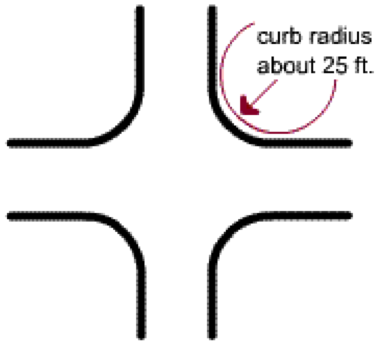
\includegraphics[width=\textwidth]{large-radius.png}
	\caption{Large Curb Radius}\label{fig:large-radius}
\end{subfigure}
\begin{subfigure}[b]{0.4\textwidth}
	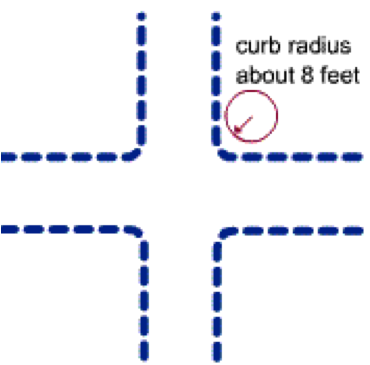
\includegraphics[width=\textwidth]{small-radius.png}
	\caption{Small Curb Radius}\label{fig:small-radius}
\end{subfigure}
\end{figure}

        The purpose of curb radii is to slow vehicles down by enabling them to make smaller turns, which ultimately reduces the risk of pedestrians being struck by vehicles when turning into a corner. Also, small curve radii can create safer intersections, improve the visibility between drivers and pedestrians, and lead to improved signal timing. By reducing the curb radii, not only will it slow down vehicles when turning, but it will also shorten the distance and time it takes for pedestrians to cross the street by nearly half of what it used to be (See Table ~\ref{table:cross-time-vs-radius} and Figures ~\ref{fig:radius-change} and ~\ref{fig:cross-time-vs-radius}).
        
\begin{figure}[h]
\centering
	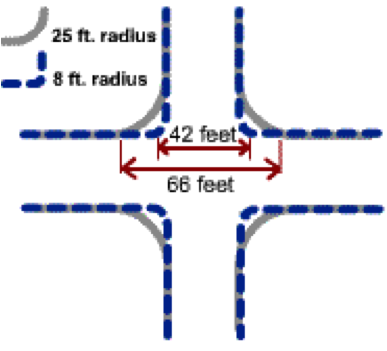
\includegraphics[scale=1]{radius-change.png}
	\caption[Effect of changing curb radius]{Change in Distance from 25ft. Radius to 8ft. Radius}\label{fig:radius-change}
\end{figure}

\begin{table}[h]
\centering
    \begin{tabular}{cc}
    Curb Radius (feet) & Average crossing time (seconds) \\ \hline
    10                 & \phantom{0}7.9                             \\
    15                 & \phantom{0}9.8                             \\
    25                 & 14.1                            \\
    \end{tabular}
\end{table}

\begin{figure}[h]
\centering
	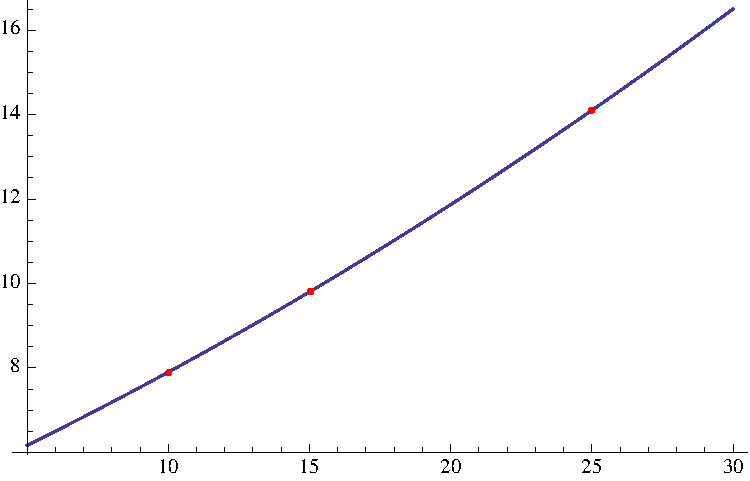
\includegraphics[scale=0.5]{cross-time-vs-radius.pdf}
	\caption[Plot of crossing times against curve radii]{A plot of the data from Table ~\ref{table:cross-time-vs-radius}}\label{fig:cross-time-vs-radius}
\end{figure}

        When streets have a large curb radius, motorists can make turns at relatively high speeds that decrease pedestrian safety. By contrast, 90-degree intersections and corners with tight curb radii tend to slow motorists down and therefore increase pedestrian safety. Motorists turning right at high speed can cut off bicyclists/pedestrians traveling straight on the arterial street. In addition, pedestrians crossing the residential street adjacent to the arterial may not expect high-speed turning traffic, or they may have their backs facing the turning cars as you can see in ~\ref{fig:back-against-car}

\begin{figure}
\centering
	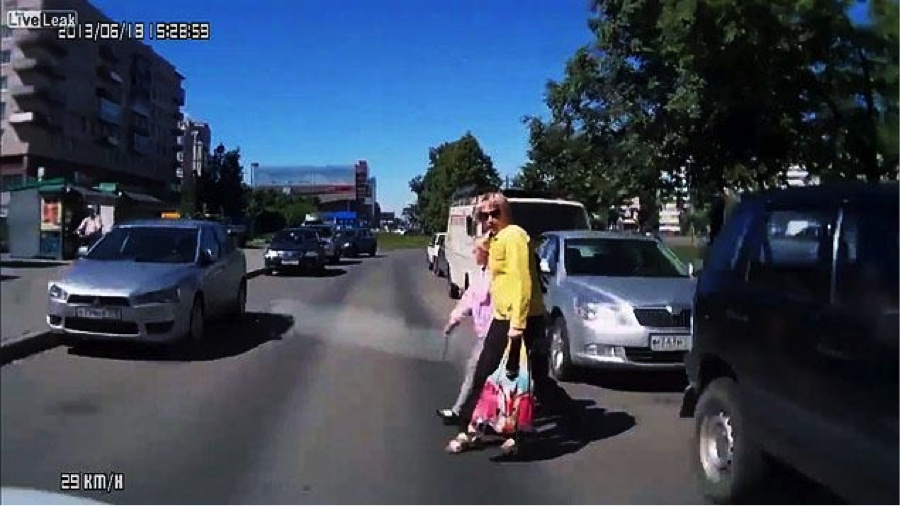
\includegraphics[width=0.5\textwidth]{back-against-car.png}
	\caption{Pedestrian Facing Back Against the Car}\label{fig:back-against-car}
\end{figure}

The cost of reconstructing tighter turning radii is in between \$5,000 to \$40,000 per corner depending on the site locations/conditions. When considering curb radii, it is important to note that in order for it to be effective, the design should meet the needs of the design vehicles with consideration for nearby land uses and prevalence of roadway users. So if there are high volumes of large vehicles making turns in a given location, a poorly designed curb radius could potentially cause the vehicles to drive over the curb and onto the sidewalk endangering pedestrians. In addition, you should always accommodate emergency vehicles, as well as school buses, and public maintenance vehicles when designing curb radii\cite{walking-info-curb}.


There is no magic number for the appropriate curb radius because it differs case by case depending on where it is located (See \figref{location-depend}). The length of the curb radius that should be used wherever possible is 5 to 10 feet, whereas an effective radius for urban streets with high volumes of pedestrians is 15 to 20 ft. For arterial streets with a substantial volume of turning buses/trucks, an appropriate effective curb radius is about 25 to 30 ft.; and the maximum desired effective curb radius is typically 35 feet for large vehicles \cite{walking-info-curb}.

\begin{figure}
\centering
	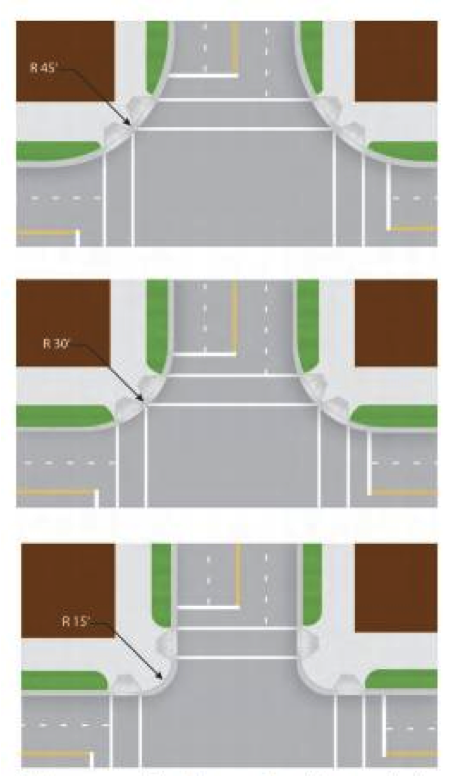
\includegraphics[scale=0.5]{location-depend.png}
	\caption{Different Curb Radii Depending on the Location}\label{fig:location-depend}
\end{figure}